\documentclass[conference]{IEEEtran}
\IEEEoverridecommandlockouts
\usepackage{cite}

\usepackage{tcolorbox}
\usepackage[colorinlistoftodos,prependcaption]{todonotes}
\usepackage{xcolor}
\usepackage{amsmath,amssymb,amsfonts}
\usepackage{algorithmic}
\usepackage{graphicx}
\usepackage{textcomp}
\usepackage{minted}
\usepackage{subcaption}
\usepackage[hidelinks]{hyperref}
\usepackage[inline]{enumitem}
\usepackage[T1]{fontenc}
\usepackage{cleveref}
\usepackage{systeme}
\setminted[scala]{baselinestretch=1,bgcolor=white,frame=single}

\def\BibTeX{{\rm B\kern-.05em{\sc i\kern-.025em b}\kern-.08em
  T\kern-.1667em\lower.7ex\hbox{E}\kern-.125emX}}


\newcommand{\unibo}{\textsc{Alma Mater Studiorum} -- \textit{Università di Bologna}}
\newcommand{\disi}{\textit{Computer Science and Engineering - DISI}}
\newcommand{\scafi}{{ScaFi}}
\newcommand{\scalaloci}{{ScalaLoci}}
\newcommand{\scafiloci}{{ScaFiLoci}}
\newcommand{\scalainline}[1]{\mintinline[fontsize=\small]{scala}{#1}}
%%%%% LEGENDA FOR NOTES %%%%%
%% RED: constraints
%% YELLOW: suggestions
%% CYAN: todos
%% GREEN: outline
\newcommand{\constraints}[1]{\todo[inline, color=red]{#1}}
\newcommand{\suggestions}[1]{\todo[inline, color=yellow]{#1}}
\newcommand{\todos}[1]{\todo[inline, color=cyan]{\textbf{TODO}: #1}}
\newcommand{\outline}[1]{\todo[inline, color=green]{#1}}
%% Utility commands
\newcommand{\round}{\texttt{round}}
\newcommand{\export}{\texttt{export}}
\sloppy
\begin{document}

\title{Towards a Machine Learning approach for Aggregate Computing} %% or Towards a Machine Learning approach for Aggregate Computing
\author{
\IEEEauthorblockN{
Gianluca Aguzzi\IEEEauthorrefmark{1},
Roberto Casadei\IEEEauthorrefmark{1},
Mirco Musolesi\IEEEauthorrefmark{1}\IEEEauthorrefmark{2},
Mirko Viroli\IEEEauthorrefmark{1}
}
\IEEEauthorblockA{\IEEEauthorrefmark{1}
\textsc{Alma Mater Studiorum}---Universit\`a di Bologna, Cesena, Italy}
\IEEEauthorblockA{\IEEEauthorrefmark{2}
University College London, London, United Kingdom\\
Email: \{gianluca.aguzzi, roby.casadei, mirco.musolesi, mirko.viroli\}@unibo.it
}}

%% Minted helpers
\definecolor{mblue}{rgb}{0.27,0.33,0.53}
%%
%% Keywords. The author(s) should pick words that accurately describe
%% the work being presented. Separate the keywords with commas.
%\begin{keywords}
%  Collective-Adaptive System \sep
%  Aggregate Computing \sep
%  Deep Learning \sep
%  Reinforcement Learning \sep
%\end{keywords}

%%
%% This command processes the author and affiliation and title
%% information and builds the first part of the formatted document.

\maketitle
\begin{abstract}
Recent trends like pervasive, autonomic, and swarm computing
 promote 
 a vision of large-scale collections of relatively simple agents
 that act and coordinate 
 with no central orchestrator
 to support distributed applications.
%
Such Collective Adaptive Systems (CAS)
 are hard to engineer,
 because mechanisms for developing global behaviour
 out of local behaviour and interaction must be devised,
 often leveraging natural inspiration.
%
In particular, in the field-based Aggregate Computing approach,
 collective adaptive behaviour is specified in terms of computational fields,
 namely maps from CAS entities to computational values evolving over time, and neighbour-based interaction.
%
However, devising efficient aggregate computing algorithms
 for different scenarios
 is not an easy task; in particular,
 a problem is determining the best local decisions based on the current context
 for fostering collective outcomes.
%
Therefore, in this work we investigate
 the possibility of using machine learning techniques
 to automatically devise local actions
 to improve existing aggregate algorithms.
%
In particular, we propose a Reinforcement Learning solution that can be seen as the first step towards the integration between Aggregate Computing and Machine Learning. 
% The goal is to improve adaptivity through low-level specifications but maintaining high-level program behaviours. 
Accordingly, we outline challenges and opportunities of this integration, and present preliminary results based on a case study where Aggregate Computing is successfully combined with Hysteretic Q-Learning.
%

\end{abstract}
\begin{IEEEkeywords}
  Collective-Adaptive System,
  Aggregate Computing,
  Deep Learning,
  Reinforcement Learning
\end{IEEEkeywords}
  
\section{Introduction}
Recent trends like pervasive~\cite{DBLP:journals/wc/Satyanarayanan01} and autonomic~\cite{DBLP:journals/computer/KephartC03} computing 
 promote a vision of artificially designed Collective Adaptive Systems (CASs)~\cite{DBLP:conf/huc/Ferscha15},
 namely collections of agents coordinating and adapting %as wholes 
 to pursue joint goals in changing environments.
% due to the increasing interconnected computational devices placed in ever-changing environments.
 Examples of CASs include robot swarms, smart cities, and digitally-augmented crowds.
%
%CASs are characterised by 
%\begin{itemize}
%\item a global order that emerges from local node interactions, 
%\item  decentralised control, and 
%\item adaptive behaviours towards environmental changes to pursuit a collective goal.
%\end{itemize}
%
CAS are notoriously hard to design and control 
 %due to as part of complex systems
 as globally desired behaviour
 has to emerge from local behaviours and interactions. 
For this reason, over the years, various approaches have tried to handle this complexity. Some of them take inspiration from the natural system composed of social animals. %--- like bees, fish, and ants. 
%
In this case, a sort of hive mind arises 
 %-- also referred to as swarm intelligence --  
 born from local interactions between agents. 
%
These kinds of behaviours are accomplished with self-organisation, 
 namely a global order that emerges from continuous 
 interactions between simple entities.

Initially, researchers had tried to translate these properties to computing systems by miming natural collective behaviour bottom-up~\cite{DBLP:journals/connection/Webb02}. %, 
 %namely trying to find the right single-node-behaviour 
 %to reach a global behaviour. %, e.g. flocking, foraging, etc.
%
However, this mapping cannot be easily defined, since we are dealing with complex systems.
%
Ideally, we would like to express collective behaviours at the ensemble level,
 abstracting over non-functional aspects such as the network topology, environment uncertainties and 
 system size.

In this direction, Aggregate Computing (AC)~\cite{DBLP:journals/computer/BealPV15} is an innovative paradigm, according to which
 developers can express collective self-organising behaviours. % through a functional program specification.
%
Indeed, an aggregate program 
 %(i.e. a program written with AC) 
 consists of the manipulation of \textit{computational fields}, a distributed
 data structure where each node is associated with the result of a computation
 performed by it.
%
%These operations are defined in \textit{field-calculus}~\cite{DBLP:conf/coordination/AudritoBDV18} --- the root of Aggregate Computing. 
% This calculus describes a set of minimal constructs to express any spatiotemporal computation.

AC captures common abstractions for collective behaviour specification in so-called ``building-blocks''. 
 %These abstractions are encapsulated in so-called ``building blocks''.
 %through which various applications have been built (e.g., for swarm robotics and crowds engineering~\cite{DBLP:journals/eaai/CasadeiVAPD21}).
However, building block synthesis concerns different stuff not only related to the behaviour itself
 but also to the "ensemble" specifications. 
 For instance, it is quite difficult to craft building blocks
 that easily adapt w.r.t. the node movements rapidity.
%
Ideally, we would like to continue building our application using these building blocks -- so the high-level specification remains the same -- but using some
 under-the-hood mechanisms that adapt the behaviour according to different environmental changes. For this reason, we claim that Machine Learning can help us in handling this "unseen" situation, leaving only the burden
 to developers of defining the right collective specifications.
%This lead to an ``hybrid" approach where a part of behaviour is still expressed using common 
% AC abstractions and another part is distilled through learning~\cite{research}.
In particular, in this paper,
 we investigate how AC can be extended with Reinforcement Learning (RL) through a case study,
 where we outline the performance improvement of the ``hop count" program ---
 i.e. an aggregate program that produces a field that stores the distance from a source zone. 
 Furthermore, we show that the learnt policy scales up to different system sizes.

The paper is divided as follow, in \Cref{background} we describe
 the AC framework, showing the context in which
 is typically applied and the overall idea of how it works, in \Cref{aggregate-and-machine-learning} we detail the relevant properties of Aggregate
 Computing in terms of machine learning problems, in \Cref{aggregate-and-rl} we describe a combination of AC with RL and then in
 \Cref{evaluation} we practically applied it in a paradigmatic AC case study,
 finally, \Cref{conclusion} we discuss the result showed and we underline a path toward an in-depth AC and RL integration.

 \section{Background and Related Work}\label{background}

%Computer Science is an incredibly evolving research area. 
% In a few years, the environment had been filled with intercommunicating computational devices, such as smartphones, smart things, and personal computers.

Collective Adaptive Systems are characterized by a very high number of nodes without a central coordinating authority that coordinate nodes. The overall behaviour is a consequence of local interactions. The systems expose self-* properties.
 
Engineering this kind of system is a thriving area, and so various approaches have been proposed.
 First attempts leverage \textit{local-to-global} techniques, where the collective behaviour emerges from local behaviour description, 
 usually inspired by nature~\cite{DBLP:journals/swarm/BrambillaFBD13}. 
%
 A natural way to describe this kind of problem is through a \textit{collective} view of the system.
 This is the idea used by the \textit{global-to-local} techniques~\cite{DBLP:journals/jlap/ViroliBDACP19,DBLP:journals/scp/AlrahmanNL20, DBLP:conf/cbse/BuresGHKKP13}, 
 where the behaviours are designed \textit{top-down}, and then the local behaviour is generated automatically from this ``system-wide'' specification. 
% 
Also, ``meet-in-the-middle''~\cite{DBLP:journals/computer/PinciroliB16} approaches exist, where
 a part of the system is still expressed bottom-up (device-centric) whereas a part is expressed top-down (swarm-centric)

In this work, we focus on Aggregate Computing~\cite{DBLP:journals/computer/BealPV15}, a global-to-local approach where
 the self-organising collective behaviour is expressed in terms of manipulation of \textit{computational fields}.
The latter could be seen as the extension of electromagnetic fields to Computer Science since it consists of a 
 map from any devices to their computational value (i.e. the result of a computation).
The computational field manipulation is ruled by \textit{field calculus}, which define the constructs needed 
 to express spatio-temporal computations~\cite{DBLP:journals/jlap/ViroliBDACP19}.
The novelty of AC consists in its composable (functional-like) system-size independent program definition: 
using basic constructs we identify the main patterns (\textit{building-blocks}) that could be reusable at the application level.
By opportunistically crafting these building-blocks it is possible to verify prominent properties such as eventual consistency %~\cite{DBLP:journals/taas/BealVPD17} 
 (i.e. the ensemble behaviour is independent of the underlying network details)
 and self-stabilisation %~\cite{DBLP:journals/tomacs/ViroliABDP18} 
 (i.e. the ability of a system to recover from arbitrary changes)~\cite{DBLP:journals/jlap/ViroliBDACP19}.

AC is studied in various simulated scenarios ranging from smart cities to crowds, 
 thanks to Alchemist~\cite{DBLP:journals/jos/PianiniMV13} (a meta-simulator for pervasive systems) and to programming languages and toolchains that support 
 this paradigm, such as ScaFi~\cite{DBLP:conf/isola/CasadeiVAD20}. %, FCCP~\cite{DBLP:conf/acsos/Audrito20} and Protelis~\cite{PianiniSAC2015}.

In the next sections, we show the field calculus operators that are essential to understand the case study presented,
 and then we underline how each node computes in order to follow the aggregate program specification.
\subsection{Field Calculus operators}
The main constructs that capture the essential aspects for programming self-organising systems are:
\begin{itemize}
  \item \textit{Stateful field evolution} expression \mintinline[escapeinside=||]{scala}{|{\color{teal}rep}|(|$e_1$|) {|($x$) => $e_2$|}} describes a field evolving in time. 
  $e_1$ is the initial field value and the function $(x) => e_2$ define how the field changes at each execution.
  \item \textit{Neighbour interaction} expression \mintinline[escapeinside=||]{scala}{|\color{teal}nbr|{|$e$|}} a view
  of the field values in the surroundings of each device where neighbours are
  mapped to their evaluations of $e$. A series of \mintinline{scala}{*hood} operators leverage this map to produce relevant result. 
  For instance, \mintinline{scala}{minHood} return the minimum value 
  within the neighbourhood.
  \item \textit{Domain partitioning} expression \mintinline[escapeinside=||]{scala}{|\color{teal}if|(|$e_0$|){|$e_1$|}{|$e_2$|}} splits the computational
  field into two non-communicating zones hosting isolated subcomputations:
  $e_1$ where $e_0$ is true, and $e_2$ where $e_0$ is false.
\end{itemize}
For a more in-depth explanation of these operators, please refer to~\cite{DBLP:journals/computer/BealPV15}.

\subsection{Computational Model}
An aggregate program execution consists of a continuously node-point execution of a \round{}, 
 that is the atomical part of AC. Each node can interact only with-in its neighbourhoods sharing the \export{}, namely the result produced by the evaluation of a \round{}.

The main round steps consist of:
\begin{enumerate}
  \item execution context creation: nodes create the execution context collecting information from the sensors, 
  the neighbourhood messages, and the old program output;
  \item program evaluation: the system-wide aggregate program is evaluated against the local context created by the nodes. 
  This produces the \export{};
  \item export sharing: the export created will be shared within the current neighbourhoods perceived by the nodes;
  \item actuations: giving the export produced, nodes may perform some actuation (e.g. motor activations, steering, ...).
\end{enumerate}

Rounds execution is completely asynchronous, so do not exist a global clock to coordinate the aggregate. 
 This makes it possible to scale easily with the node number size. This collective, proactive and periodical execution will eventually lead to the satisfaction of the system-wide specification.

\section{Aggregate Computing and Machine Learning}\label{aggregate-and-machine-learning}

In this section, we analyse the characteristics of the AC paradigm,
 map these to relevant machine learning contributions in the literature,
 and point out different learning perspectives about the integration of AC with Machine Learning

\paragraph{Multi-and many-agent system}
%
An aggregate system is a multi-agent system
 and, often, a \emph{many}-agent system
 where a large number (hundreds or more)
 of autonomous entities are programmed to achieve 
 some collective behaviour through \emph{repeated} 
 sensing, computation, communication, and actuation steps.
%
Due to the high stochasticity of the environment,
 it is almost impossible to know and
 program the optimal behaviour for all agents in advance.
 This uncertainty results in the need of creating intelligent agents
 so that they can learn the optimal behaviour and adapt to environmental changes.
%
In recent decades there has been an emerging trend in the use of RL 
 in multi-agent settings -- called Multi-Agent Reinforcement Learning (MARL) -- as a powerful, robust and adaptive learning paradigm.
 Progress has been considerable and a wide range of algorithms are now available.

MARL is a conjunction of Game theory and RL, 
 and there are several (even orthogonal) viewpoints on which researchers have been focused.

First attempts from RL viewpoint, 
 goes towards a so-called \textit{independent learning}~\cite{DBLP:journals/tsmc/BusoniuBS08} approach, 
 where each agent learn locally against the whole environment~\cite{DBLP:conf/icml/Tan93}.

Examples of these are Hysteretic Q-Learning (used to reduce non-stationarity)~\cite{hysteretic-q}, 
 Lenient Learning~\cite{DBLP:journals/jmlr/WeiL16}, and Frequency Maximum Q-value~\cite{DBLP:conf/atal/KaisersT10}.
%
The pro of these approaches is that their complexity does not scale up with the number of agents, 
 but, unfortunately, the learning process is extremely non-stationary and unstable.
% 
Furthermore, they are heuristic and do not exist any convergence proof (even if, in practice, they often reach a good policy).

Other efforts have focussed on achieving equilibria such as Nash-equilibrium of Pareto optimality.
 The first works towards this direction are Nash-Q-Learning~\cite{nash-q}, Friend-or-Foe Q-learning~\cite{DBLP:conf/icml/Littman01}, Minimax-Q~\cite{DBLP:conf/icml/Littman94}.
The problem is that it is used with few agents and scale hardly with the application complexity.
%
Finally, current emerging trends tend to leverage a so-called centralised training and decentralised execution (CTDE) approach, by which 
 agents should leverage the system-wide knowledge at training time but at runtime, they act independently~\cite{DBLP:journals/aamas/Hernandez-LealK19}.
 Most promising approaches in this direction are MAPPO~\cite{DBLP:journals/corr/abs-2103-01955}, COMA~\cite{DBLP:journals/corr/FoersterFANW17} and MADDPG~\cite{DBLP:conf/nips/LoweWTHAM17}.
 
The main problem with most of the solutions available in the literature is that they consider a small number of agents (or at least test them on small games).
 In AC instead, we need to find a technique that does not depend on the system node count.

\paragraph{Neighbour-based or indirect (environment-mediated) interaction}
%
In aggregate systems, a device can directly interact only with its neighbours.
%
Data flows may be implemented
 to support indirect communication across multiple hops;
 however, information from devices far away tends to be obsolete.
%
The environment can also be used, via stigmergy~\cite{DBLP:journals/scp/NicolaSI20},
 for indirect communication;
 however, a device can typically only access 
  to a very local portion of the environment.
%
In other words, the system state is only \emph{partially observable}.
In practice, CTDE technique aims to solve these problems, using a \emph{global} view at training time but
 a \emph{partial view} at execution time.

Furthermore, when the system node size is very large, novel works of Mean-Field Reinforcement Learning~\cite{DBLP:conf/ijcnn/ZhouZX21} are able to
 handle learning efficiently, reasoning about agent and agent neighbourhoods.
%
\paragraph{Learning goal: collective behaviour}
%
The devices of an aggregate 
 must cooperatively learn the ``aggregate program'',
 namely the collective behaviour 
 that achieves a particular \emph{global goal}
 in a decentralised, resilient way.
%

% \paragraph{Self-organisation, swarm robotics} it is condensed it other perspective, so I think it is better to avoid this paragraph.
%
% \suggestions{You can talk about similar problem structure (i.e. the collective follow the same local behaviour)}

\paragraph{Emergent behaviour}
%
The collective behaviour of an aggregate system
 \emph{emerges} 
 from a dense network of computations and interactions
 in an evolving environment.
%

Typically, in CAS, single-agent RL brings to emergent behaviour and is used in various applications~\cite{DBLP:conf/icse/DAngeloGGGNPT19}.

\paragraph{Delayed, global rewards}
%
In the light of the above properties,
 if we consider a learning approach based on rewards,
 we must observe that such rewards would be
 delayed and mostly global---i.e.,
 it may not be easy to solve the credit assignment problem
 to distinguish good from bad individual contributions
 to the global outcome.

A way to handle this kind of rewards in multi-agent settings is \textit{difference rewards}~\cite{DBLP:conf/atal/DevlinYKT14, DBLP:conf/aaai/FoersterFANW18}. It is used to capture agents contributions to the system's global performance.
\paragraph{Transient phase}
%
When an aggregate behaviour is carried out,
 we often focus on the final stable outcomes after the transitory period.
%
However, intermediate results are also important,
 and invariants should hold throughout the entire computation.

\paragraph{Dynamic topology}
%
If we admit \emph{mobility} and \emph{failure} (rarely considered in related works, where node population is fixed),
 then we must also consider
 the possibility of changes in neighbourhoods
 and hence the need of dealing with dynamic topologies.

\subsection{Integrating Learning Mechanisms into Aggregate Computing}
We now outline the different perspectives about AC with learning, 
 to clarify the current and the future research path.
%
\paragraph{Application} Learning can be useful at different levels in our framework.
 First of all, learning can be applied to the building blocks definition.
% 
Indeed, most of our results and applications are based on them.
%
The building block improvement may consist either of learning a correction factor or by entirely learning the behaviour.

On the other side, learning can be useful also for framework related stuff,
 mainly aiming at "non-functional" aspects. 
 Trust mechanisms, evaluation frequency, energy consumption manager, package storage are all the things that could take advantage of using Machine Learning algorithms.
 
\paragraph{Learning problem} 
The learning problem in multi-agent settings can be posed as \textit{Independent} and \textit{Team} learning. 
In the foster, each agent perform the learning process and while in the latter,
 the learning process is performed only by one agent and then shared with the collective (in a typical CDTE setting).
% 
Team learning is usually used in the ``swarm'' system, due to the homogeneous behaviour 
 --- i.e. each agent performs the same program. 
 Here, a common reward signal exists and evaluate the overall collective behaviour.
% 
In AC, each agent follows the \textit{same} aggregate program shared within the entire system, so Team learning can 
 be applied seamlessly.

On the other hand, Independent Learning is usually applied in Collective
 (Self-)Adaptive System \cite{csas-and-marl}.

In particular, Independent Reinforcement Learning reach good results in this kind of system, 
 even if no theorem exists as in the single-agent context.
%
With Independent learning is still possible to reach a global collective behaviour convergence. 
 Indeed using a common reward signal, the collective may reach the same behaviour through emergence \cite{iima2008swarm, nguyen2018swarm}.

\paragraph{Learning technique}
Aside from what kind of problem we set up, we can then use different Machine Learning techniques,
 such as RL or Supervised Learning (SL).
%
SL is rare in CSAS -- or in the ``swarm" like system in general.
%
Novel works~\cite{DBLP:conf/corl/TolstayaGPP0R19} leverage Graph Neural network to learn how agents should communicate, 
 supposing to know the right behaviour (i.e. produced via global vision simulation or by emulation of natural phenomena).

In AC, S) can be applied when we want to build up new building blocks from zero. 
% 
Indeed, we eventually know the right state of the system, but we do not know how the system can reach it.

RL is predominantly used in CAS, 
 due to its flexibility and thanks to the plethora of approaches used in this scenario~\cite{csas-and-marl}.

In our case, RL can be used both at the building block level and the framework level.
%
For the foster, the simplest scenario can be that agents learn a correction factor to improve a long-term reward signal.
 
\paragraph{Learning time}
Finally, learning can be performed \textit{offline}, \textit{online} or \textit{offline an then online} (\textit{mixed time}).
% 
The foster is the common scenario in multi-agent settings.
 Here indeed, we can leverage simulation to know the right computational field and then use one of the novels CTDE techniques. 
Mixed-time learning can be a mid-level complexity direction instead.
 Here, simulation can always be exploited to reach a good behaviour, but at runtime, 
 the behaviour can be adapted based on the new environmental situations. 
Finally, we can imagine that learning can be performed online. 
 It is a common situation where we do not know the environment and also simulation can be very hard to accomplish. 
 In mixed and online cases, RL is the most suitable model, because agents \textit{learn by doing}.

\section{Aggregate Computing with Reinforcement}\label{aggregate-and-rl}
\begin{figure}
  \centering
  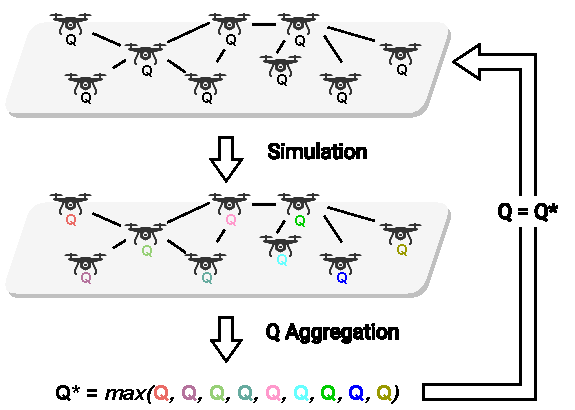
\includegraphics[width=\linewidth]{img/algorithm-learning.pdf}
  \caption{This figure shows the main steps of RL in AC.
  Each agent starts with his copy of a Q table. 
  Then, during the simulation, they refine them Q tables changing q values according to their experience (different colours mean different values). 
  In the end, a new $Q_{max}$ table will be created aggregating each agent table. 
  Finally, a new episode starts using this $Q_{max}$ as a starting Q table.
  }
  \label{fig:aggregate-q-learning}
\end{figure}
As first experiments, we leverage RL to improve building blocks. 
% 
In this section, we briefly describe how RL can be injected into the computation loop,
 and what RL we used with AC.

From a local view, program execution can be seen as:
$$
f : \textit{Context} \rightarrow \textit{Output}
$$
Where $\textit{Context}$ contains:
\begin{itemize}
  \item $\sigma(name) \rightarrow \textit{data}$: a function from sensor name to the perceived value;
  \item $\phi(\textit{ID}) \rightarrow \textit{Export}$: a function from id to neighbourhoods export data.
\end{itemize}
The computational field $\theta$ contains all output produced by the system.

Speaking of RL settings, we need to define the state function and the reward function.
%
The execution needs to be distributed, so the state will be a function from the local node context:
$$
K := \Omega(\textit{Context})
$$

Reward function instead, might be depending on the learning technique, time and problem. 
 Indeed, if we perform learning offline, it could be defined from the overall \textit{simulated} computational field:
$$
\textit{R}_{global} := \psi({\theta})
$$
If we use an online mode, it needs to be defined as a function to the local node context:
$$
\textit{R}_{local} := \psi(\textit{Context})
$$
Finally, actions influence the current aggregate program output, changing the program evaluation as:
$$
f_{rl} : \textit{Context} \rightarrow \lambda(\textit{Output}, \textit{Action})
$$
As remarked before, the policy $\pi$ need to be distributed, so each agent can choose the action that will be performed:
$$
\textit{Action} \leftarrow \pi(K)
$$

As a first step towards a complete integration between AC and RL, we decide to set up an Independent learning technique, 
 by which each agent try to improve our current local policy (shown in \Cref{fig:aggregate-q-learning}). 
% 
We made this choice inspired by other work in CSAS~\cite{csas-and-marl} and swarm systems~\cite{nguyen2018swarm}.

Our approach is partially inspired by Swarm Q-Learning~\cite{nguyen2018swarm} and leverage Hysteretic Q-Learning~\cite{hysteretic-q} to 
 handle the non-stationarity in the environment.
%
In particular, each agent maintains a local Q table ($Q_i(s, a)$, where $i$ is the agent id) following the standard hysteretic update:
$$
\delta \leftarrow r + \gamma * max_a Q_i(s', a) - Q_i(s_t, a_t)
$$
$$
Q(s_t, a_t) =  \begin{cases} 
  Q(s_t, a_t) + \alpha * \delta & \mbox{if } delta >= 0 \\ 
  Q(s_t, a_t) + \beta * \delta & \mbox{otherwise }
\end{cases}
$$

At the end of the episodes, each agent has collected its local experience, which can vary in different zones. So, 
 we combine the N (the number of nodes) Q table selecting the maximum value for each state-action pair since we assume a homogeneous behaviour:
$$
Q_{max}(s, a) = max_i(Q_i(s, a))
$$
Then, in the next episode, each agent starts with the $Q_{max}$ and try to refine it.
\section{Evaluation}\label{evaluation}
\begin{figure*}[h]
  \centering
  \begin{subfigure}[b]{0.32\textwidth}
      \centering
      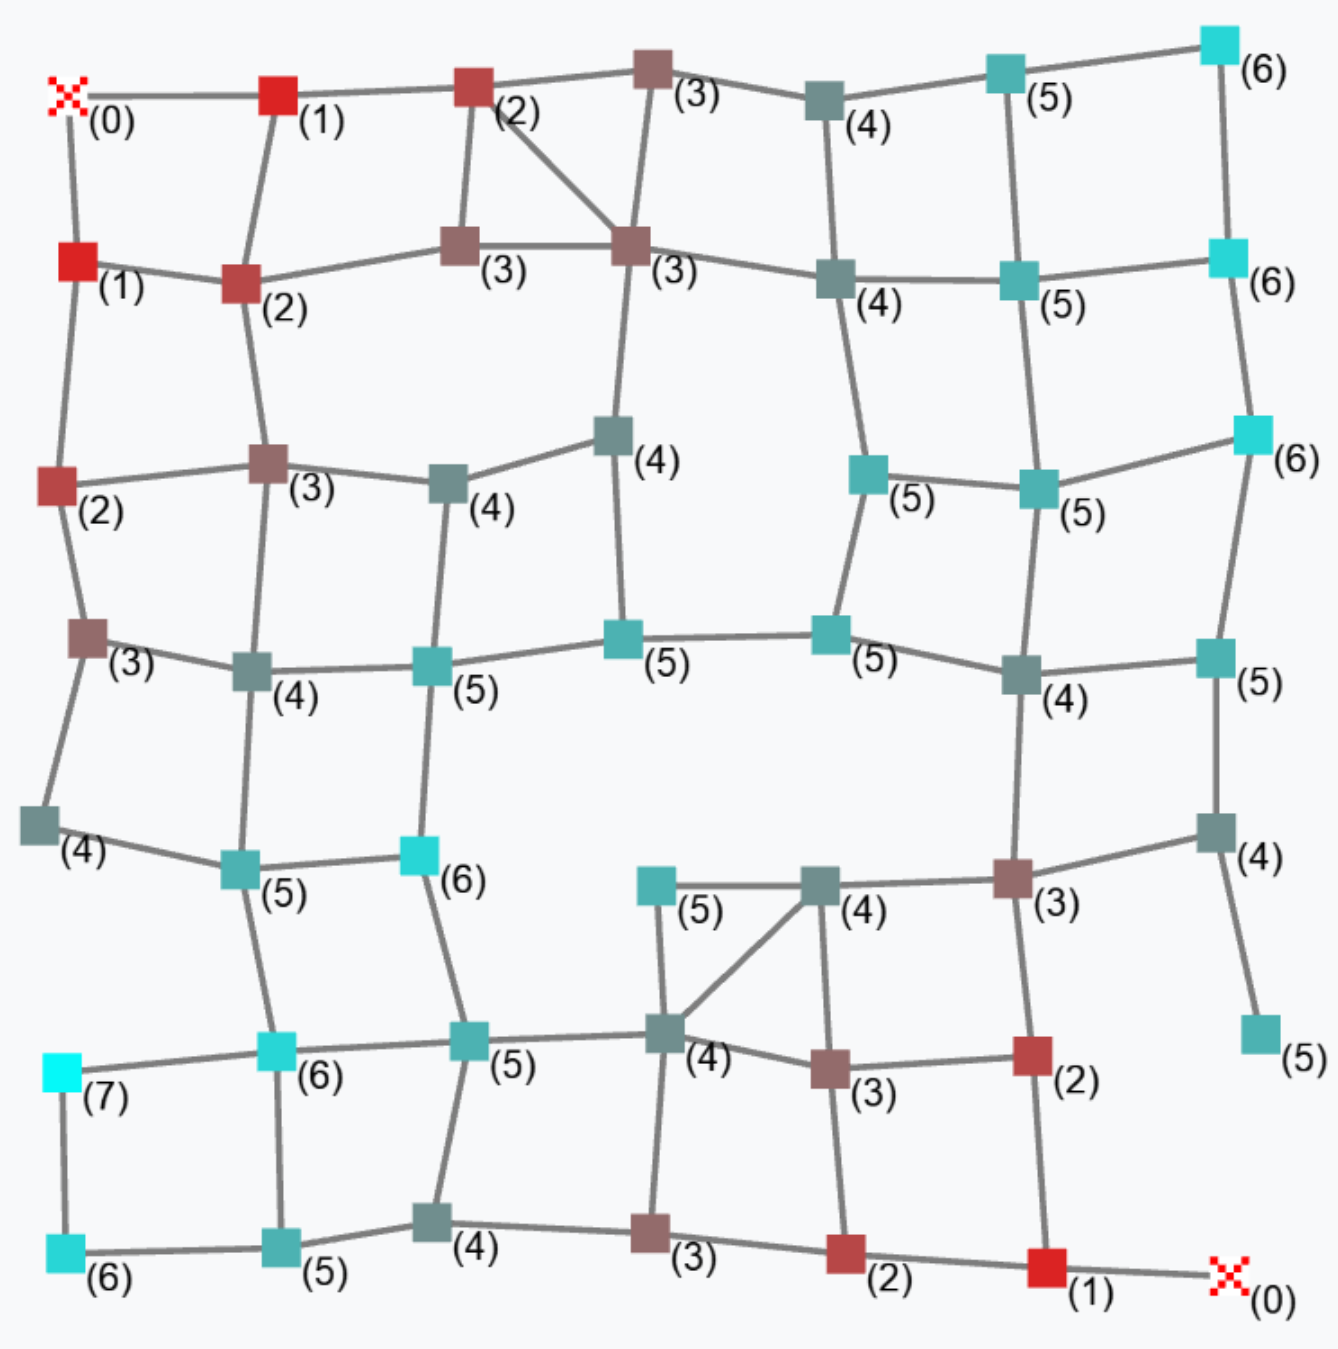
\includegraphics[width=\textwidth]{img/hop-count-1.png}
      \caption{Stable situation: Two source nodes exists}
  \end{subfigure}
  \hfill
  \begin{subfigure}[b]{0.32\textwidth}
      \centering
      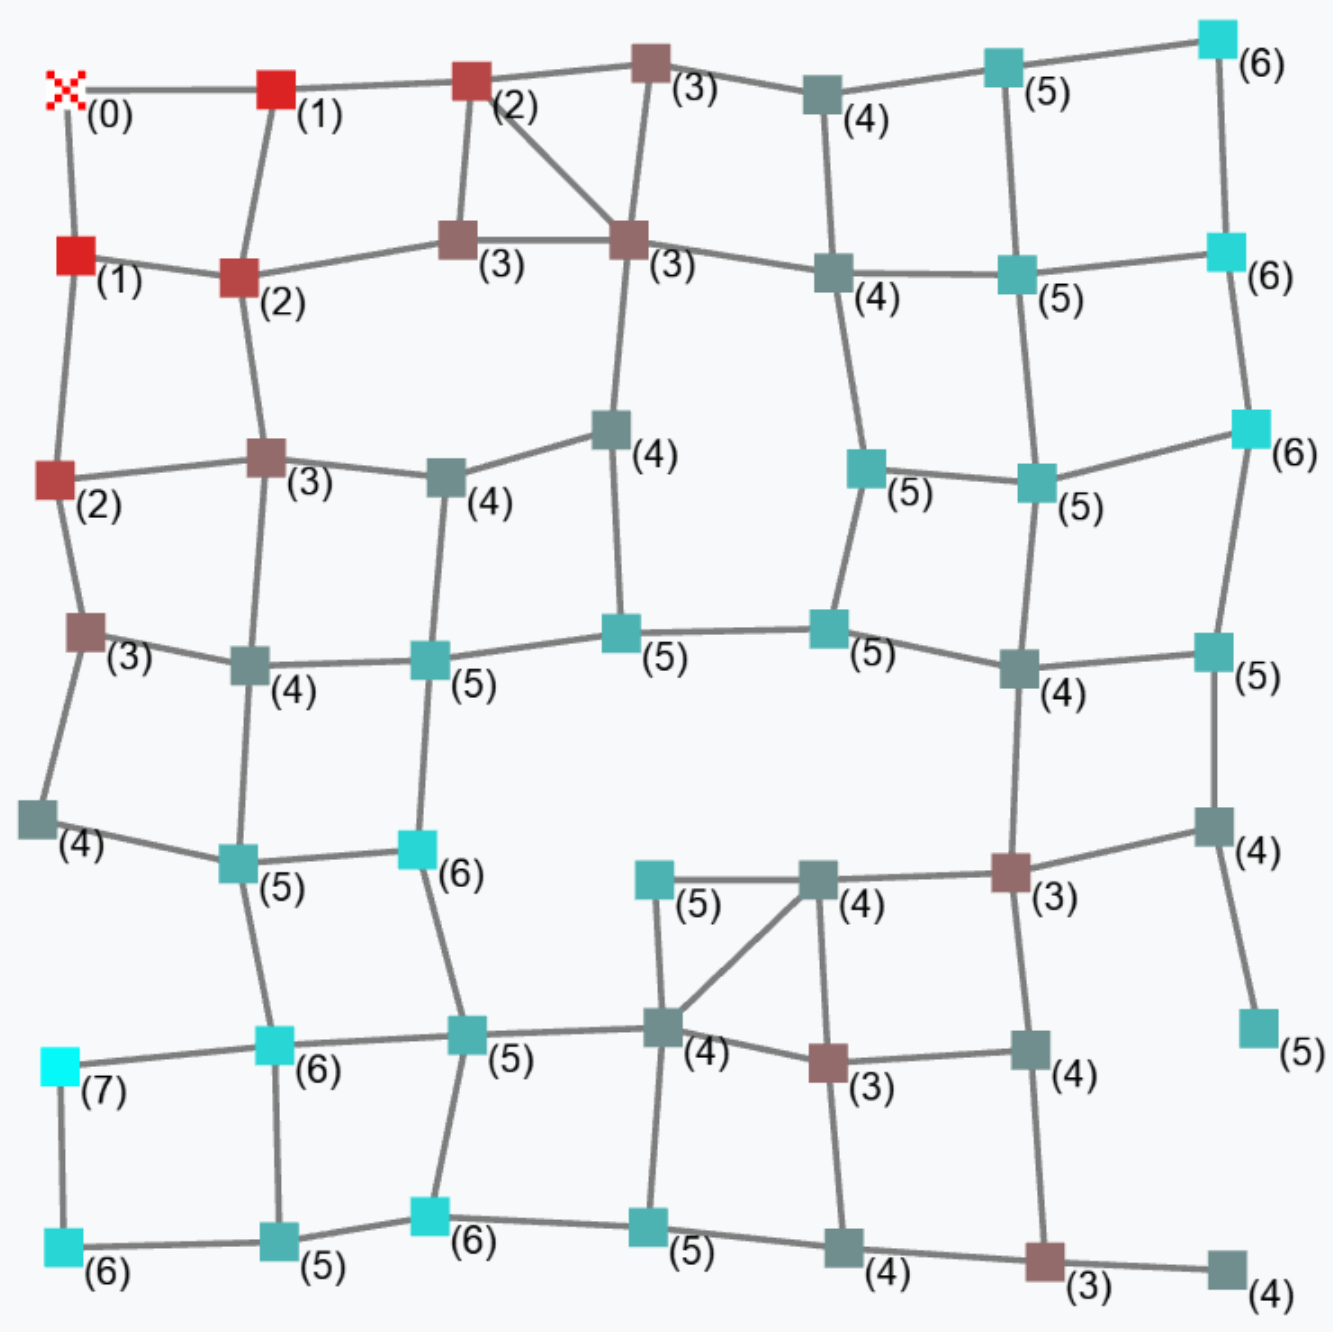
\includegraphics[width=\textwidth]{img/hop-count-2.png}
      \caption{Unstable situation: One source disappears}
  \end{subfigure}
  \hfill
  \begin{subfigure}[b]{0.32\textwidth}
      \centering
      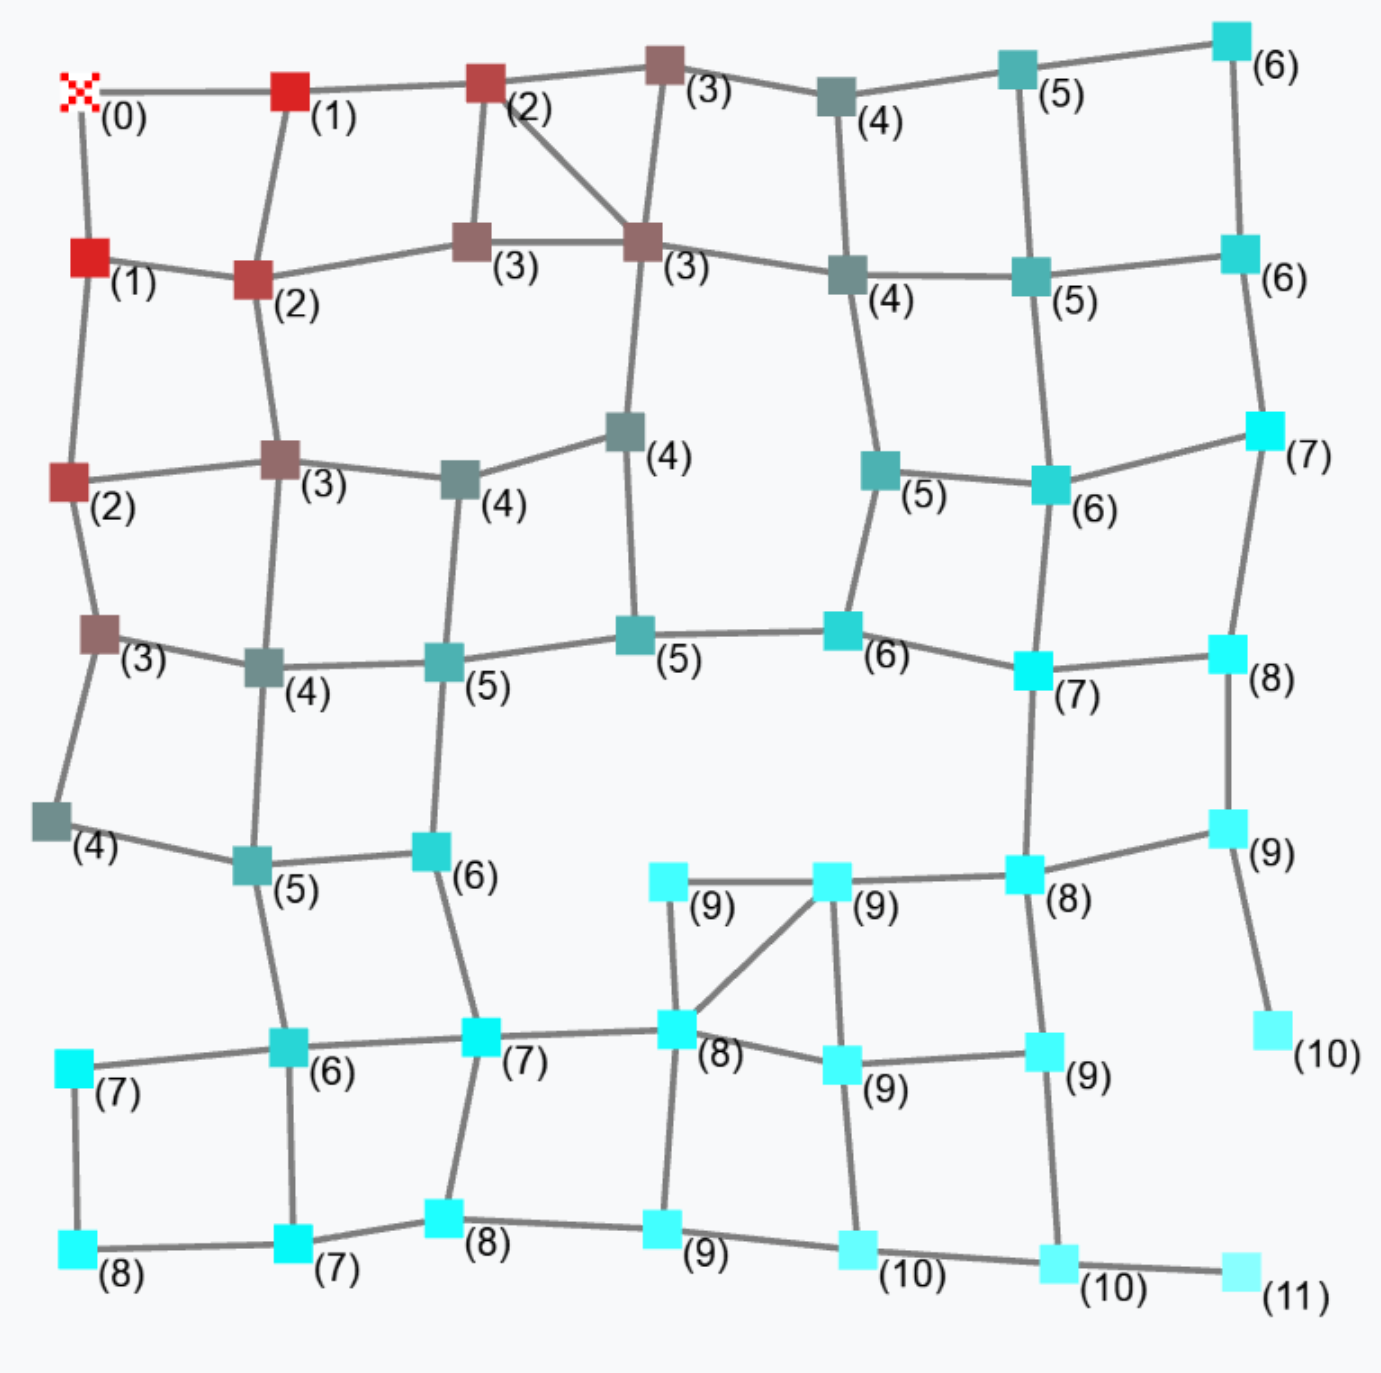
\includegraphics[width=\textwidth]{img/hop-count-3.png}
      \caption{Stable state reached}
  \end{subfigure}
  \caption{Graphical result of hop count evaluation. The node with a red cross is the target zone. The label 
  associated with each node is the result of the aggregate program evaluated in that zone.}
  \label{fig:hop-count}
\end{figure*}
In this section, we outline the results of the application of RL for one simple
 aggregate program: the hop count. In this case, the computational field that will eventually be produced consists of the distance in terms of the minimum number of nodes needed to reach source nodes ((\Cref{fig:hop-count})).

A naive implementation of this kind of problem can be described in AC as:
\begin{minted}[fontsize=\scriptsize]{scala}
def hopCount(): Int = {
  rep(Double.PositiveInfinity) { 
    hopCounts => mux(source) 
    { 0 } 
    { minHoodPlus(nbr{hopCounts}) + 1 }
  }
}
\end{minted}
However, this solution suffers from the slow-rising problem~\cite{DBLP:conf/saso/AudritoCDV17}. 
 It consists of a slow convergence time when an equilibrium situation is broken.
So, our first intuition is to accelerate convergence through learning.
 In particular, the previous solution can be rewritten as:

 \begin{minted}[fontsize=\scriptsize]{scala}
def hopCountRl(k: Int, w: Int): Int = 
{
  rep(Double.PositiveInfinity) { 
    hopCounts => 
      val currentState = 
        state(hopCounts, k, w)
      val action = localPolicy(state)
      hopCout() + action
  }
}
\end{minted}

Where the actions are discrete values (0, 1, 2 in our experiments) that correct the local result following a policy refined through learning.
%
The state instead, is built upon previous output and of the neighbourhoods output.
 In particular, in this case, it is built from a temporal window in order to encode the hop count velocity:
\begin{minted}[fontsize=\scriptsize]{scala}
def speed(hopCount: Int, k: Int) =
{
  val min = minHood(nbr{ hopCounts })
  val window = recentValues(min, k)
  min - window.head 
}
\end{minted}
\mintinline{scala}{recentValues(data, k)} is an aggregate operator that returns a list containing the last k data perceived by the agent.
Then, due to the partial observability of the environment, we maintain a 
 list of velocity, to understand the hop count direction:

 \begin{minted}[fontsize=\scriptsize]{scala}
def state(hopCount: Int, k: Int, w: Int) =
{
  val currentSpeed = speed(hopCount, k)
  recentValues(currentSpeed, w)
}
\end{minted}

Where \textbf{\texttt{k}} and \textbf{\texttt{w}} are two parameters of this algorithm.
%
The policy is learnt locally, during simulation, using our version of Q-Learning algorithm. 
 The reward function consists in: 
\[
\systeme*{0 : & \mbox{\textit{hop count output is right}}, -1 : & \mbox{\textit{otherwise}}}
\]
The idea is to maintain the nodes in a stable situation or to
 fasten the time needed to reach a stable one.
%
\Cref{fig:aggregate-learning-loop} shows the learning loop in details.
\begin{figure}
  \centering
  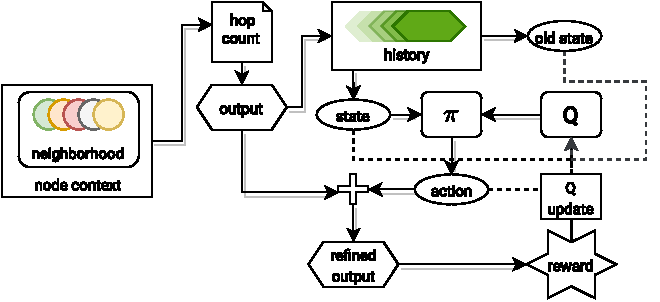
\includegraphics[width=\linewidth]{img/aggregate-program-evaluation.pdf}
  \caption{Each agent, starting from their context, 
  periodically performs the standard hop count. 
  Using the output produced and the history of state and output, 
  each agent computes its current state. 
  Using it, they evaluate the action to speed up the hop count convergence following a policy. 
  This new refined output is then used to evaluate the reward and to refine the Q table (dotted line path)}
  \label{fig:aggregate-learning-loop}
\end{figure}
%\begin{minted}[obeytabs=true,tabsize=1]{scala}
%val inf = Double.PositiveInfinity
%rep((initState, initPolicy, inf)) {
%  (oldState, policy, hopCount) => 
%      val currentState = 
%        state(hopCount, k, w)
%      val action = policy(state)
%      val output = mux(source) 
%        { 0 } 
%        { minHood(hopCount) 
%          + 1 
%          + action
%        } 
%      }
%      val currentReward = 
%        reward(output)
%      val improvedPolicy = 
%        qLearning(oldState, 
%          state, 
%          action, 
%          reward,
%          policy
%      (currentState, policy, output)
%    )
%}
%\end{minted}

\subsection{Simulation Setup}
We verify our learning algorithm through simulation~\footnote{repository at \url{https://github.com/cric96/alpaca-2022-ac-rl}} leveraging Alchemist and ScaFi.
 To check if the aggregate eventually speeds up the hop count convergence time, we create a situation where the rising problem emerges (\Cref{fig:hop-count}):
 in the beginning, two source nodes exist in the network, ($A$ and $B$).
 At the time $t$, $B$ disappears. So the nodes near $B$ start a slow process
 to eventually reach the distance towards $A$.
We use 80 ($N$) nodes displaced into an irregular grid with a width of 100 meters and a height of 20 meters. 
 Each node has a neighbourhoods range equal to 8 meters --- on average, each node has 7 neighbours. 
 The time $t$ is fixed to 20.
 Each simulation episode lasts 60-time unit. Finally, we set $k = 3$ and $w = 2$.
% 
We train the aggregate for 500 episodes.
 The Q-learning parameters are:
$$ 
\alpha = 0.5,
\beta = 0.05,
\gamma = 0.9
$$
Furthermore, we use a $\epsilon$ decay policy for the $\epsilon$-greedy policy as:
\begin{equation*}
  \begin{array}{l}
    \epsilon_t = \epsilon_{start} * e^{-t/\theta}\\ 
    \epsilon_{start }= 0.99, \theta=4000
  \end{array}
\end{equation*}
In doing so, the agent will explore the state-action space as much as possible.

\Cref{fig:simulation}-a shows the error for both naive implementation and RL-based implementation as time changes.
The error is evaluated as:
\begin{equation*}
  \begin{array}{l}
    error(i, t) \leftarrow  | \textit{rightValue}(i,t) - \textit{output}(i,t) | \\
    total_{error} = \frac{1}{T} * \sum_{i = 0}^T \frac{1}{N} * \sum_{j = 0}^N = error(i, j)
  \end{array}
\end{equation*}

where \textbf{i} is the node identifier and \textbf{t} is the time when the error is evaluated.
%

Then, we test our learnt algorithm in different environments (\Cref{fig:simulation} b,c,d). To do that, we share the learnt Q-table to the 
entire aggregate and we test the program changing the system size (80, 360 and 760 nodes).
For each population size, we run 50 episodes and then we average the error at each time step. 
As a result, the aggregate speed-up convergence in each new situation.

\begin{figure*}
  \begin{subfigure}[b]{\textwidth}
    \centering
    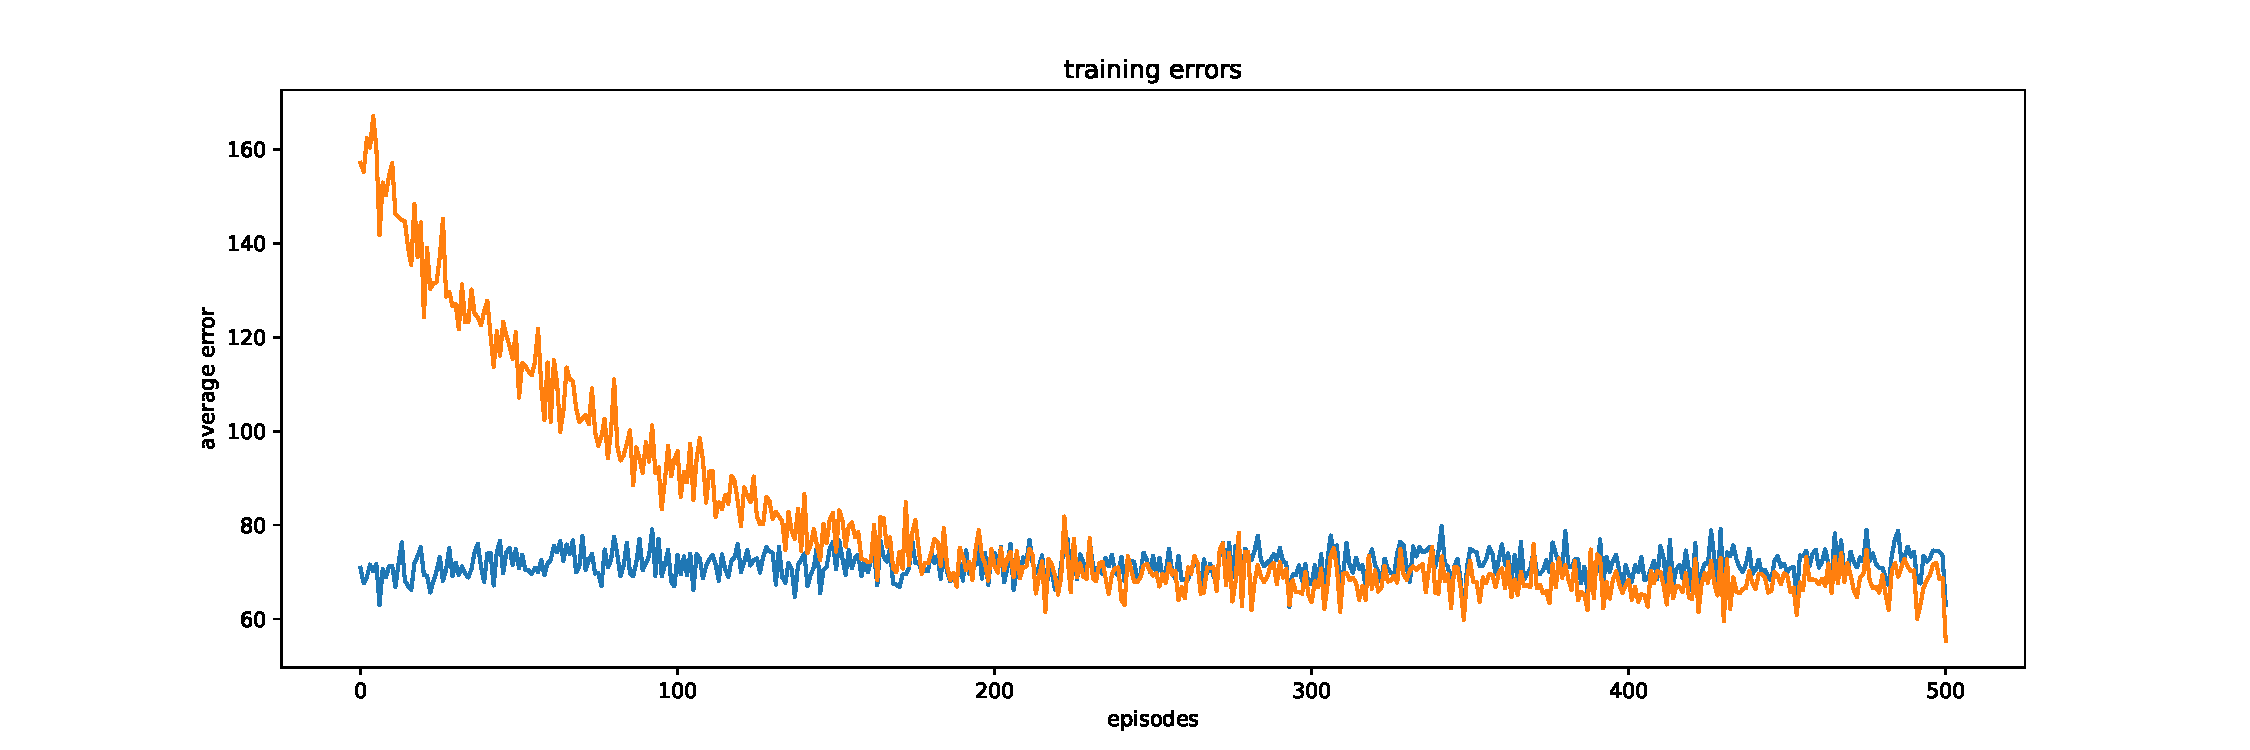
\includegraphics[width=\textwidth]{img/mean-error}
    \caption{The \textit{orange} line 
    describes the RL solution error. The \textit{blue} line shows
    the naive solution error.}
    \hspace{5mm}
    \label{fig:simulation-a}
  \end{subfigure}
  
  \centering
  \begin{subfigure}[b]{0.3\textwidth}
      \centering
      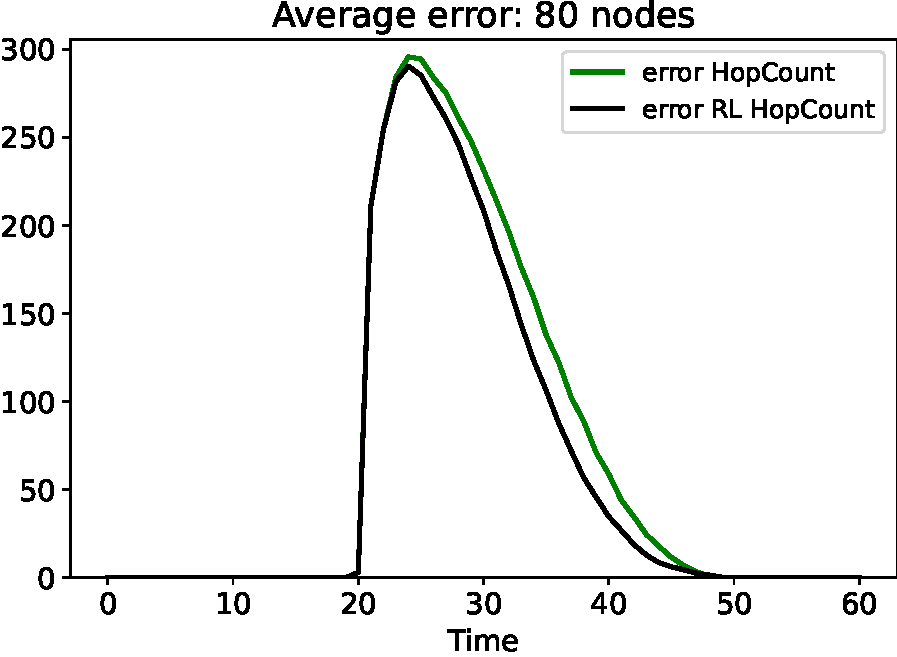
\includegraphics[width=\textwidth]{img/80}
      \caption{}
      \label{fig:simulation-b}
  \end{subfigure}
  \hfill
  \begin{subfigure}[b]{0.3\textwidth}
      \centering
      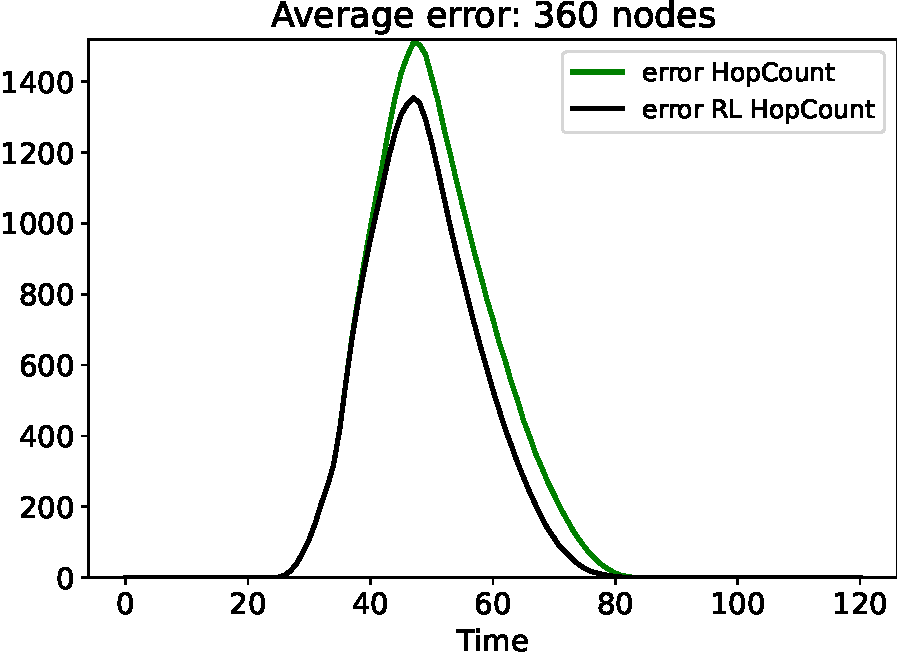
\includegraphics[width=\textwidth]{img/360}
      \caption{}
      \label{fig:simulation-c}
  \end{subfigure}
  \hfill
  \begin{subfigure}[b]{0.3\textwidth}
      \centering
      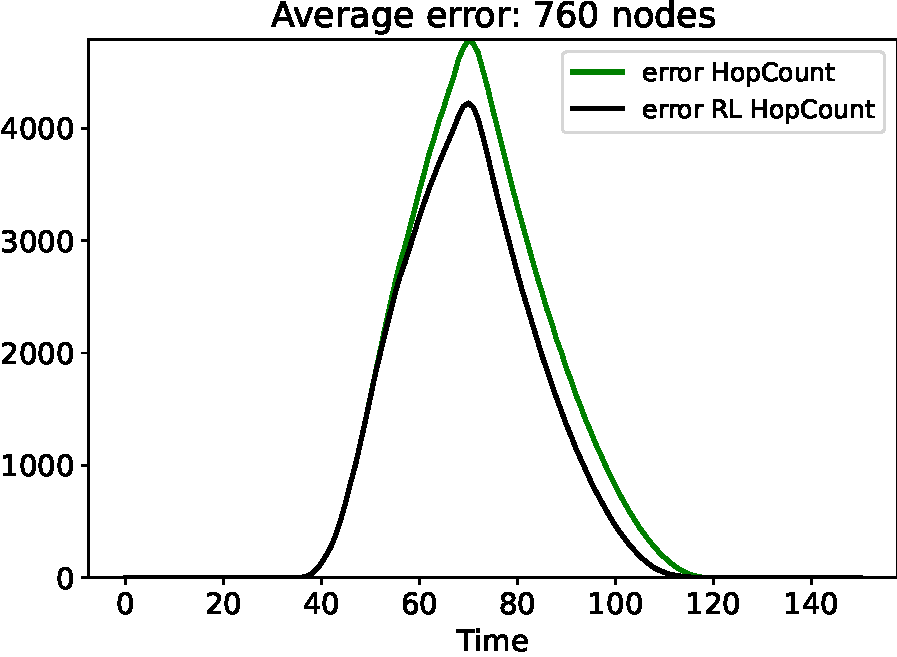
\includegraphics[width=\textwidth]{img/760}
      \caption{}
      \label{fig:simulation-d}
  \end{subfigure}
  \caption{Analysis of the learning process. \Cref{fig:simulation-a} shows the $total_{error}$ evolution during the learning process. \Cref{fig:simulation-b}, \Cref{fig:simulation-c}, and \Cref{fig:simulation-d} show the average error in three different simulations with 80, 360 and 760 nodes. 
  The black line is the error of the RL-based solution, 
  the green line is the error produced by the standard hop count implementation.}
  \label{fig:simulation}
\end{figure*}
%\todos{add blinking scenarios}
%\todos{add movement scenarios}

\section{Discussion and Concluding Remarks}\label{conclusion}
In this article, we have discussed the combination of AC with Machine Learning techniques in order to improve adaptivity
 and effictveness of the AC framework.
In doing so, we compared AC problems with current Machine Learning solutions in MASs systems.
%
Finally, we explore the combination of AC with RL (in particular Hysteretic Q-Learning).
RL application in this kind of settings is quite an explored -- even if some works exists~\cite{DBLP:conf/icml/YangLLZZW18} -- 
 area for several reason, such us the highly system dynamic, non-stationarity,  partial enviroment observability, and non-bounded system size.
In a case study we empirically shown the effictveness of RL, by which we speed up the convergence time of
 aggregate program taking in consideration -- the hop count.
Furthermore, we have shown that the learnt program can easily scale up to system size.

This is a first effort towards an ``hybrid'' collective programming approach, where the high-level program specification is 
 done by a designer and the low-level matters are leaved to machine learning algorithms.

We know that this is preliminary work and it shed light on several problems that we should handle in the future.

Aggregate systems are partially observable from the perspective of each node. 
 Local observations may not be statistically significant in summarising the state of the entire aggregate. 
 In the future, we could address this problem through recurrent networks and a CTDE learning methodology.
 
The learning, in this case, was applied at the building block level. 
 Another possible direction is to use it at the framework level, e.g., to select which messages to send to the neighbourhood or not. 
 This has already been addressed in the literature, usually under the name of \textit{learn to communicate}~\cite{DBLP:journals/corr/abs-1908-03963}. 
 A novel way to handle this problem is to use Graph Neural Networks~\cite{DBLP:journals/corr/abs-1812-08434} to learn the representation of a distributed system and to select messages based on that representation. 
 Thus, we should consider this methodology when we will extend RL at the AC framework level.
 
In this case, we applied a variation of the independent learning approach. 
 Agents first learn the best policy locally, and then at the end of the episode, a learner merges the Q-tables. 
 However, this does not reduce the problems of scalability and non-stationary, since a central agent must still collect all the Q-tables of the aggregate. 
 In particular, to handle the scalability issues, we will have to consider decentralised approaches based only on the neighbourhood information (or local leaders).
 
Finally, we do not address the multi-agent credit assignment problem in this work. 
 Indeed, we use a global reward function for the whole aggregate. In this way, however, learning often degenerated because it was difficult to understand the influence of an agent w.r.t. the system. 
 To reduce this problem, we will consider novel techniques of difference reward~\cite{DBLP:conf/atal/AgoginoT04} or counterfactual baseline~\cite{DBLP:journals/corr/FoersterFANW17}.

\bibliographystyle{IEEEtran}
\bibliography{biblio}
%%
%% If your work has an appendix, this is the place to put it.
%\appendix

\end{document}

%%
%% End of file
